\documentclass[twocolumn,showpacs,
    nofootinbib,aps,superscriptaddress,
    eqsecnum,prd,showkeys,10pt,floatfix]{revtex4}
\setlength{\paperheight}{11in}
\usepackage{amssymb}
\usepackage{amsmath}
\usepackage{graphicx}
\usepackage{dcolumn}
\usepackage{hyperref}
% Keywords command
\providecommand{\keywords}[1]
{
    \small
    \textbf{\textit{Keywords---}} #1
}
\begin{document}
\begin{titlepage}
    \title{An optimal linear approach to cruise controlling a fixed-wing aircraft in the presence of wind}
    \author{Bogdan I Boboc, Eva H Dulf}
    \affiliation{Faculty of Automation and Computer Science, department of Automation and Applied Informatics, Technical University of Cluj-Napoca, Romania}

    \begin{abstract}
        Linear Gaussian control (LQG) is a well suited control strategy when it comes to stabilize systems under a fixed set of operating conditions around an equilibrium point.
        It provides a great mechanism to ensure a stability margin for any real system with a high degree of non-linearity.
        It has been successfully used in conjugation with a system composed of states defined in different scales.
        This paper aims to develop a control strategy for a fixed wing aircraft which operates in windy conditions at a cruise altitude, focusing on the case of a small scale Unmanned Aerial vehicle (UAV) with no access to any wind sensors, thus relying on an estimator to identify the wind's intensity and direction.
        This approach seems really promising especially when paired with a gain-scheduling mechanism.
    \end{abstract}
    \keywords{Autopilot, Linear Quadratic Control, Aerospace, Fixed-Wing Aircraft}
    \maketitle
\end{titlepage}
\newpage


%%%        S  S    E  E E        C     T T T T T    0       O       N        N
%%%     S          E           C           T        I     O   O     N  N     N
%%%        S       E  E E    C             T        I   O       O   N    N   N
%%%           S    E           C           T        I     O   O     N      N N
%%%     S S        E  E  E       C         T        I       O       N        N
\section{Introduction}
This research proposes a control strategy for a small aircraft flying in windy
conditions, with a lack of weather sensors, based on a linear Gaussian control
and using an estimator to make up for the lack of sensors. It will walk through
all the stages of development for such a controller and present the reader will
all the necessary information for conducting a similar research in order to
compare results between approaches when different parameters are taken into
consideration. It will try to prove the strategy by simulating the aircraft in
windy conditions and giving it a path to follow.
\par
While there has been a strong trend to automate flight in the recent years in
both military and civil fields, as presented in {{\cite{lessons}}}, we can see
that the market for low computational power solutions is still wide open. While
studies like {{\cite{Gain_Scheduled}}} and {{\cite{UTC}}} do a great job for
solving the problem of autonomous flight, using different control structures,
they both rely heavily on a ground station with a high degree of computational
power available. This is a very common, but this study aims to develop a low
power controller, placed on board of the aircraft, yielding similar results.
\par
This study is divided into 8 sections. The first section is the Introduction,
while the second section focuses on the frames of reference used when
developing the dynamic model of our system. The third and forth chapters focus
on the mathematical model and incorporating the effects of wind into the
differential equations. In the fifth section we will describe the implemented
control structure that aims to keep the aircraft in the air and estimate the
wind disturbances, while the sixth chapter will deal with ensuring a null
steady state error when using a predefined path even when wind is present. In
the last chapter the testing results will be listed and the conclusion of the
study will be drawn.

%%%        S  S    E  E E        C     T T T T T    0       O       N        N
%%%     S          E           C           T        I     O   O     N  N     N
%%%        S       E  E E    C             T        I   O       O   N    N   N
%%%           S    E           C           T        I     O   O     N      N N
%%%     S S        E  E  E       C         T        I       O       N        N
\section{System of reference}
In order to apply Newton's equations of motion to the location and orientation
of an aircraft when examining its dynamics, an appropriate inertial coordinate
system must be used. Additionally, it is necessary to specify relative
locations and velocities using multiple frames of reference, with the choice of
which frame to use being a matter of convenience. A coordinate system fixed on
the surface of the Earth is preferred to construct the velocity equations
because sensors like the Global Positioning System (GPS) measure the aircraft's
velocity in relation to the Earth. The information provided by the
accelerometer and the gyroscope are specific to the system of reference fixed
on the body of the vehicle. In light of this a second frame of reference shall
be used, namely the body frame, which is fixed on the body of the aircraft
itself.

%%%        S  S   U       U  B B       S  S    E  E E        C     T T T T T    0       O       N        N
%%%     S         U       U  B   B    S        E           C           T        I     O   O     N  N     N
%%%        S      U       U  B B        S      E  E E    C             T        I   O       O   N    N   N
%%%           S     U   U    B   B        S    E           C           T        I     O   O     N      N N
%%%     S S           U      B B      S S      E  E  E       C         T        I       O       N        N
\subsection{Body-fixed and inertial frames of reference}
Solving a dynamic problem requires an inertial reference frame, $F^I$, which is
a system of reference fixed or in a uniform rectilinear translation relative to
the distant stars. Meeting this requirement leads to the possibility of using
the Newton's second law for the motion of a particle, which relates the
external forces acting on the particle to its mass and acceleration relative to
$F^I$. Generally, the rotation of the Earth is neglected in the analysis of the
flight dynamics when flying happens on small distances. Therefore, any
coordinate frame with the origin at a defined location on the Earth can be used
as an inertial frame. Let $F^E$ denote the Earth-fixed reference, frame having
the origin close to the launching location, it's X axis indicating North, it's
Y axis indicating East, and it's Z axis indicating vertically. This coordinate
system will further be used in order to describe the aircraft's position and
orientation relative to a fixed point on the earth's surface. In order to use
ignore Coriolis effect we will work in a flat-earth environment. The origin of
the body fixed frame, depicted as $F^B$, coincides with the vehicles center of
gravity. The x-axis of this frame will always be pointing through the nose of
the aircraft, the y-axis will be pointing through the right wind, and the z
axis will be pointing downwards. The body-fixed reference frame, $F^B$, has an
angular velocity of $\varPhi$ in relation to $F^I$, depicted as
$\varPhi={[p,q,r]}^T$.
\par
The propulsive force acts along x-axis of the body-fixed system and the
aerodynamic forces are described by a vector having its center in the
aerodynamic center of the aircraft. We will assume that the aerodynamic center
of the aircraft and the center of gravity overlap, to simplify the model. The
interaction of forces will be analyzed in this body fixed system, because it
makes it is the native system for most of the forces present during flight.
Furthermore, some onboard sensors, specially the inertial measurement unit,
collect data in this particular frame.
\par
The Euler angles, used to describe the three sequential rotations around the z
y x axes, that can be used to describe the orientation of $F^B$ with relation
to $F^I$, are noted as $(\phi,\theta,\psi)$. Yaw$(\phi)$, pitch$(\theta)$, and
roll$(\psi)$ angles rotate the airplane's body around the x, y and z-axes
respectively. The transformations that describe the rotations are:
\begin{align}
    R_1(\phi) & = \begin{bmatrix}
                      1 & 0           & 0          \\
                      0 & \cos(\phi)  & \sin(\phi) \\
                      0 & -\sin(\phi) & \cos(\phi)
                  \end{bmatrix}
    \label{PhiEulerRotation}
\end{align}
\begin{align}
    R_2(\theta) & = \begin{bmatrix}
                        \cos(\theta)  & 0 & \sin(\theta) \\
                        0             & 1 & 0            \\
                        -\sin(\theta) & 0 & \cos(\theta)
                    \end{bmatrix}
    \label{thetaEulerRotation}
\end{align}
\begin{align}
    R_3(\psi) & = \begin{bmatrix}
                      \cos(\psi)  & \sin(\psi) & 0 \\
                      -\sin(\psi) & \cos(\psi) & 0 \\
                      0           & 0          & 1
                  \end{bmatrix}
    \label{PsiEulerRotation}
\end{align}
This allows us to define the complete rotational matrix from $F^I$ to $F^B$ as:
\begin{align}
    R_{BI} & =R_1(\phi)R_2(\theta)R_3(\psi)
    \label{BodyToEarthRotationMatrix}
\end{align}

%%%        S  S   U       U  B B       S  S    E  E E        C     T T T T T    0       O       N        N
%%%     S         U       U  B   B    S        E           C           T        I     O   O     N  N     N
%%%        S      U       U  B B        S      E  E E    C             T        I   O       O   N    N   N
%%%           S     U   U    B   B        S    E           C           T        I     O   O     N      N N
%%%     S S           U      B B      S S      E  E  E       C         T        I       O       N        N
\subsection{Wind axes coordinate frame}
The wind reference frame, $F^W$ has the same point of origin like the
body-fixed frame, namely the center of gravity of the aircraft. As depicted his
x-axes is rotated around the body x body axis so that it aligns with the
velocity vector of the aircraft. The y-axis also reflects that by being rotated
around the z-axis of the aircraft with an angle of sideslip $\beta$. The z-axis
still points down, but now it has also been rotated around the y-axis with the
same $\alpha$ angle, formerly known as the angle of attack of the vehicle, just
like the x-axis. This frame will later be used to describe the aerodynamic
forces acting upon our aircraft. The wind vector can also be denoted in the
inertial reference frame and his components would be $\omega_{w}={[p_w, q_w,
            r_w]}T$. The rotation matrix from body to wind reference frames can be defined
as follows:
\begin{align}
    R_{WB} & =\begin{bmatrix}
                  C(\alpha)C(\beta) & -C(\alpha)S(\beta) & -S(\alpha) \\
                  S(\beta)          & C(\beta)           & 0          \\
                  S(\alpha)C(\beta) & S(\alpha)S(\beta)  & C(\alpha)
              \end{bmatrix}
    \label{WindToBodyRotationMatrix}
\end{align}
where $S(\phi)$ denotes sin and $C(\phi)$ denotes the cosine of the angle $\phi$.


%%%        S  S    E  E E        C     T T T T T    0       O       N        N
%%%     S          E           C           T        I     O   O     N  N     N
%%%        S       E  E E    C             T        I   O       O   N    N   N
%%%           S    E           C           T        I     O   O     N      N N
%%%     S S        E  E  E       C         T        I       O       N        N
\section{Modelling an aircraft}
This section derives the mathematical model of our aircraft. It will be
considered as a rigid body with six degrees of freedom. The Earth is considered
flat and still for the purpose of simplicity, making $F^E$ a Newtonian frame of
reference $F^I$. As long as the distances are close enough to the radius of the
earth, we can assume the air density as constant, it should be emphasized that
this approximation holds true for the majority of flight altitudes, that were
taken into consideration for our small aircraft. The equations of motion are
firstly derived under the presumption that the atmosphere is at rest with
respect to the Earth, and the wind effect is then appropriately taken into
account. The presentation in this section is mainly based on
    {\cite{Aircraft_Control_and_Simulation}},
{\cite{Dynamics_of_Atmospheric_Flight}},
{\cite{Field_Path_Following_for_Miniature_Air_vehicles}} textbooks.

%%%        S  S   U       U  B B       S  S    E  E E        C     T T T T T    0       O       N        N
%%%     S         U       U  B   B    S        E           C           T        I     O   O     N  N     N
%%%        S      U       U  B B        S      E  E E    C             T        I   O       O   N    N   N
%%%           S     U   U    B   B        S    E           C           T        I     O   O     N      N N
%%%     S S           U      B B      S S      E  E  E       C         T        I       O       N        N
\subsection{State variables}
The motion of an airplane in relation to the Earth can be represented by
position, direction, velocity, and angular velocity. The position of the
aircraft center of gravity in the inertial coordinate frame will be indicated
by the vector $P_E$, whose elements are $P_E={[p_N,p_E,p_D]}^T$. The real
altitude of the vehicle will be equal to the inverse of the down position
element $h=-p_D$ to account for the fact that the system's z-axis is pointing
downward and to provide parallelism with the body-fixed reference frame when
the latter is not rotated. As a result, the position of the airplane at any
given time with respect to an inertial point of reference can be expressed as:
\begin{align}
    P & = \begin{bmatrix}
              p_N \\
              p_E \\
              -p_D
          \end{bmatrix}
    \label{PostionVectorInInertialMatrixWithInverseDownComponent}
\end{align}
\par
The Euler angles denote the angles needed in the equation
    {\ref{BodyToEarthRotationMatrix}}. Thus, we can define the vector:
\begin{align}
    \varPhi & = \begin{bmatrix}
                    \phi   \\
                    \theta \\
                    \psi
                \end{bmatrix}
    \label{EulerAnglesVector}
\end{align}
where $\phi,\theta,\psi$ represent the rotation angles between the body-fixed frame $F^B$ and the inertial reference $F^I$ around the $x^B,y^B,z^B$ axis.
\par
The inertial velocity vector $V_E$ of an aircraft is widely represented in a
variety of coordinate systems. Its constituents are provided by:
\begin{align}
    {V_E}={R_{EW}V_W}={R_{EB}V_B}
    \label{VelocityRotationEquation}
\end{align}
where
\begin{align}
    {{V_E}=\begin{bmatrix}
                   v_n \\
                   v_e \\
                   v_d
               \end{bmatrix}}
    {{V_w}=\begin{bmatrix}
                   V_a \\
                   0   \\
                   0
               \end{bmatrix}}
    {{V_B}=\begin{bmatrix}
                   v_u \\
                   v_v \\
                   v_w
               \end{bmatrix}}
    \label{TrueAirspeed}
\end{align}
where $v_n$, $v_e$, $v_d$ denotes the velocity of the aircraft in the earth-fixed frame on the north, east down axis respectively. $V_a$ stands for the true airspeed in the wind frame and $v_u$, $v_v$, $v_w$
denotes the velocity of the aircraft along the x, y, z-axis of the body frame respectively. The rotation matrices can be calculated starting from {\ref{BodyToEarthRotationMatrix}} and {\ref{WindToBodyRotationMatrix}} as such:
\begin{align}
    {R_{EW}}={R_{WE}}^T \\
    {R_{EB}}={R_{BE}}^T \\
    {R_{BW}}={R_{WB}}^T \\
    {R_{EW}}={R_{EB}R_{BW}}
    \label{MatrixRotationEquation}
\end{align}
The true airspeed $V_a$ denotes the aircraft's velocity vector relative to the surrounding air, with the components $V_a={[u,v,w]}^T$.
If the atmosphere is at rest, a scenario that we will use for modelling without taking into consideration the effect of wind. The true airspeed will be equal to the aircraft's velocity relative to the fixed reference frame $F^I$.
The equation that describes the true airspeed in the body reference frame is written below:
\begin{align}
    {V_a}^B={V_b}={R_{WB}V_W}
    \label{TrueAirspeedMatrixForm}
\end{align}
this equation can be written more explicitly as:
\begin{align}
    {\begin{bmatrix}
             u \\
             v \\w
         \end{bmatrix}}=V_a{\begin{bmatrix}
                            \cos(\alpha)\sin(\beta) \\
                            \sin(\beta)             \\
                            \sin(\alpha)\cos(\beta)
                        \end{bmatrix}}
    \label{TrueAirspeedComplete}
\end{align}
Since we are just expressing the same value in a different reference frame its module should remain the same, this means:
\begin{align}
    {\lvert V_a \rvert}=\sqrt{v^2+u^2+w^2}
    \label{TrueAirspeedModule}
\end{align}
In order to rotate from the wind reference frame to the body reference frame, the angles of attack $\alpha$ and sideslip $\beta$ have to be expressed relative to known states, thus:
\begin{align}
    {\alpha}=\arctan{\frac{w}{u}}
    \label{AlphaFormula}
\end{align}
\begin{align}
    {\beta}=\arctan{\frac{v}{V_a}}
    \label{BetaFormula}
\end{align}
The angular velocity vector can be represented as $\omega={[p,q,r]}$ in the body-fixed and wind-axes coordinate frames.
Where $p$, roll rate, stands for the angular velocity around the $x^b$ axis, $q$, pitch rate, stand for the angular velocity around the $y^b$ axis and $r$, yaw rate, stands for the angular velocity around the $z^b$ axis.
This measure can also be defined in the wind reference frame using the rotation matrix $R_{BW}$ as shown below:
\begin{align}
    \omega_w=R_{BW}\omega=\begin{bmatrix}
                              p_w \\
                              q_w \\
                              r_w
                          \end{bmatrix}
    \label{AngularVelocityInWind}
\end{align}
\par
Thus the state vector can be described as a column vector formed from the
vectors described before. Thus, the state vector:
\begin{align}
    X^T={\begin{bmatrix}
             V_B     \\
             \omega  \\
             \varPhi \\
             p_E
         \end{bmatrix}}
        ={\begin{bmatrix}
                  u      \\
                  v      \\
                  w      \\
                  p      \\
                  q      \\
                  r      \\
                  \phi   \\
                  \theta \\
                  \psi   \\
                  p_n    \\
                  p_e    \\
                  p_h
              \end{bmatrix}}
\end{align}
Then, in {\cite{Equations_of_Motion}}, the equations of motion for a rigid body aircraft when assuming a stationary flat-Earth and the atmosphere at rest are given, and they take the form:
\begin{align}
    {\dot{V_B}}={-{\Omega_B}{V_B}+R_{BE}\times{g_0}+\frac{F_B}{m}}
    \label{VelocityInInertialFrame}
\end{align}
\begin{align}
    {\dot{\varPhi}}={\varsigma(\varPhi)\omega}
    \label{AngularAccelerationInInertialFrame}
\end{align}
\begin{align}
    {\dot{\omega}}={-{J}^{-1}{\Omega_B}{J}\omega+J^{-1}T_B}
    \label{AngularVelocityInInertialFrame}
\end{align}
\begin{align}
    {\dot{p_E}}={R_{BE}V_A}
    \label{PositionInInertialFrame}
\end{align}
$\Omega_B$ is the cross-product of the body angular rates, $g_0$ is the gravitational acceleration measured at sea level.
$F^B$ is the equivalent force acting on the aircraft's center of gravity, basically the sum of all forces considered in the model.
$m$ is the mass of the aircraft and $J$ stands for the inertial matrix of our vehicle.
The term $T^B$ stands for the net torque acting on the vehicle.
As will be shown later, the whole mathematical model presented in {\ref{PositionInInertialFrame}},{\ref{AngularAccelerationInInertialFrame}},{\ref{VelocityInInertialFrame}} and {\ref{AngularVelocityInInertialFrame}} can be divided into translational and rotational equations.

%%%        S  S   U       U  B B       S  S    E  E E        C     T T T T T    0       O       N        N
%%%     S         U       U  B   B    S        E           C           T        I     O   O     N  N     N
%%%        S      U       U  B B        S      E  E E    C             T        I   O       O   N    N   N
%%%           S     U   U    B   B        S    E           C           T        I     O   O     N      N N
%%%     S S           U      B B      S S      E  E  E       C         T        I       O       N        N
\subsection{Force and moments equations}
The forces and moments operating on the aircraft center of gravity drive the
last two equations derived in {\ref{VelocityInInertialFrame}}. They have both
components as a result of a variety of causes, the most important of which are
the propulsive and aerodynamic impacts.
\par
The propulsive and aerodynamic components, $F_p$ and $F_a$, can be used to
describe the force vector from equation {\ref{VelocityInInertialFrame}} like
this:
\begin{align}
    F_b=F_p+F_a
    \label{SumOfAerodynamicAndPropulsionForces}
\end{align}
The effects of the thrusters can be found in the translational equations in the form of $F^B$ and in the rotational equations in the form of $T_B$.
The engine thrust, represented in vector form as $\vec{T}$, represents the propulsive force generated by the propellers.
Generally, the engines are positioned along the aircraft's longitudinal body axis so that the resultant force has only one not null component in the body-fixed reference frame pointing in the direction of the x-axis, i.e.

\begin{align}
    F_p=\begin{bmatrix}
            T \\\\
            0 \\\\
            0
        \end{bmatrix}
    \label{ThrustInPropulsionVector}
\end{align}
The aerodynamic force can be described in both body and wind axes. Regardless of whether frame is used, the components are connected by the rotation matrix {\ref{WindToBodyRotationMatrix}}.
To make the equations look cleaner lift (L), drag (D), and side force (Y) are specified in the wind axes.
\begin{align}
    {F_a}^W=\begin{bmatrix}
                -D \\\\
                Y  \\\\
                -L
            \end{bmatrix}=
    \begin{bmatrix}
        \bar{q}S{C_D} \\\\
        \bar{q}S{C_Y} \\\\
        \bar{q}S{C_L} \\\\
    \end{bmatrix}
    \label{AerodynamicForceInTermsOfDynamicPressureInTheWindFrame}
\end{align} where S is the wing area, $C_D,C_L$ and $C_Y$ are physical coefficients that depend on the angle of attack, angle of sideslip and the practical design of the aircraft, which will be discussed later, and $\bar{q}$ is the free-stream dynamic pressure described by the formula:
\begin{align}
    \bar{q}=\frac{\rho(h){V_a}^2}{2}
\end{align}
where $\rho(h)$ is the dynamic static atmospheric pressure at the attitude $h$. They can be represented in terms of body-axes dimensionless aerodynamic coefficients $C_x,C_y,C_z$ by denoting the components of the aerodynamic force in the body axes by $(X_a,Y_a,Z_a)$:
\begin{align}
    F_a=\begin{bmatrix}
            X_a \\\\
            Y_a \\\\
            Z_a
        \end{bmatrix}=
    \begin{bmatrix}
        \bar{q}S{C_x} \\\\
        \bar{q}S{C_y} \\\\
        \bar{q}S{C_z}
    \end{bmatrix}
    \label{AerodynamicForceInTermsOfDynamicPressureInTheBodyFrame}
\end{align}
or in terms of the aerodynamic force's wind axis components:
\begin{align}
    \begin{bmatrix}
        X_a \\\\
        Y_a \\\\
        Z_a
    \end{bmatrix}=
    \begin{bmatrix}
        -D{C(\alpha)}{C(\beta)}-Y{C(\alpha)}{S(\beta)}+L{S(\alpha)} \\\\
        -D{S(\alpha)}+Y{C(\beta)}                                   \\\\
        D{S(\alpha)}{C(\beta)}-Y{S(\alpha)}{S(\beta)}-L{C(\alpha)}
    \end{bmatrix}
    \label{AerodynamicBodyCoefficientsDefinedInTermsOfAerodynamicForces}
\end{align}
It is obtained by extending the force equation {\ref{VelocityInInertialFrame}} and inserting the above notations:
\begin{align}
    \begin{bmatrix}
        \dot{u} \\\\
        \dot{v} \\\\
        \dot{w}
    \end{bmatrix}=
    \begin{bmatrix}
        rv-qw-g_0\sin(\theta)+\frac{X_a+T}{m}          \\\\
        -rv+qw+g_0\sin(\phi)\cos(\theta)+\frac{Y_a}{m} \\\\
        qu-pv+g_0\cos(\phi)\cos(\theta)+\frac{X_a+T}{m}
    \end{bmatrix}
    \label{AccelerationInInertialFrameDiffEquation}
\end{align}
The system of a rigid body aircraft flying through a still atmosphere can be expressed into a 12 state highly coupled differential model with a great degree of non-linearity. This expression can be derived from {\ref{VelocityInInertialFrame}}, {\ref{AngularAccelerationInInertialFrame}}, {\ref{AngularVelocityInInertialFrame}}, and {\ref{PositionInInertialFrame}}.
Note that for both the navigation and force equations given in  {\ref{AerodynamicForceInTermsOfDynamicPressureInTheBodyFrame}}, two alternates have been presented {\ref{AerodynamicForceInTermsOfDynamicPressureInTheWindFrame}}.
Although not directly visible in these equations, the control vector determines the thrust force and deflections of the moveable surfaces that manage the aerodynamic forces ${(D, L, Y)}$ and moments ${(\bar{L},  M,  N)}$.
\par
The mathematical model created by putting these equations together is
predicated on the following assumptions:
\par
\begin{enumerate}
    \item The aircraft is a rigid body with a plane of symmetry.
    \item The Earth will be considered as a flat earth with no movement relative to
          far-off stars.
    \item There is no wind in the surround atmosphere.
\end{enumerate}

%%%        S  S    E  E E        C     T T T T T    0       O       N        N
%%%     S          E           C           T        I     O   O     N  N     N
%%%        S       E  E E    C             T        I   O       O   N    N   N
%%%           S    E           C           T        I     O   O     N      N N
%%%     S S        E  E  E       C         T        I       O       N        N
\section{Flying in a turbulent environment}
In this chapter we will revise the effects of wind on our aircraft, and an
estimating strategy will be outlined in order to overcome our lack of pressure
sensors in our scenario.

%%%        S  S   U       U  B B       S  S    E  E E        C     T T T T T    0       O       N        N
%%%     S         U       U  B   B    S        E           C           T        I     O   O     N  N     N
%%%        S      U       U  B B        S      E  E E    C             T        I   O       O   N    N   N
%%%           S     U   U    B   B        S    E           C           T        I     O   O     N      N N
%%%     S S           U      B B      S S      E  E  E       C         T        I       O       N        N
\subsection{Wind description}
We initially define wind as a component of the velocity field that the aircraft
flies in order to understand and research how air motion impacts the system.
The air mass is continually moving as a result of solar heating, Earth
rotation, and other thermodynamic and electromagnetic processes. The velocity
vector of the atmosphere is often variable in space and time and has a mean
value and variations. Atmospheric turbulence or gust is the remaining
fluctuating proportion, while mean wind is the steady-state velocity at a
certain point.
\par
The wind is used mostly for navigation and direction, whereas turbulence
predominantly impacts airplane stability. $\vec{W}$ is the traditional notation
for the air mass's velocity vector relative to the Earth. The overall velocity
field within the atmosphere is defined as follows based on the above
considerations:
\begin{align}
    \vec{W}=\vec{W_M}+\vec{W_F}
\end{align}
\par
where $\vec{W_M}$ is the mean wind vector and $\vec{W_F}$ is the atmospheric
turbulence.
\par
The north, east, and down velocity components of local wind are expressed in
the direction of the Earth-fixed reference frame by $W_n$, $W_e$, and $W_h$,
respectively. The transformation matrices produced in the previous section can
be reused to represent the air mass velocity vector in various coordinate
systems for convenience.
\par
Therefore:
\begin{align}
    \vec{W}=\begin{bmatrix}
                W_n \\\\
                W_e \\\\
                W_h
            \end{bmatrix}=
    \begin{bmatrix}
        W_{n_M}+W_{n_F} \\\\
        W_{e_M}+W_{e_F} \\\\
        W_{h_M}+W_{h_F}
    \end{bmatrix}
    =R_{WB}\begin{bmatrix}
               u_w \\\\
               v_w \\\\
               w_w
           \end{bmatrix}
\end{align}
\par
where ${(u_w, v_w, w_w)}$ represent the wind components in the body-fixed
reference frame and $R_{IB}$ is given by equation
    {\ref{MatrixRotationEquation}}.
\par
A mathematical model of such disturbances is required to investigate the wind
vector effect on an aircraft's the flight qualities. Complete wind cannot be
represented deterministically; in other words, it cannot be expressed using
analytical formulations. The wind field, on the other hand, can be treated as a
stochastic process with statistical features. The random-process theory is
heavily used in the development of a wind gust model, and the reader is
directed to {\cite{Gust}} for a thorough discussion on the issue.
\par
The Dryden wind turbulence model, often known as Dryden gusts, is a
mathematical model of continuous gusts approved for use in certain aircraft
design and simulation applications by the US Department of Defense.
    {\cite{Field_Path_Following_for_Miniature_Air_vehicles}} The Dryden model
handles continuous gusts linear and angular velocity components as spatially
variable stochastic processes, with each component's power spectral density
specified. Due to the rational power spectral densities of the Dryden wind
turbulence model, precise filters that take white noise inputs and output
stochastic processes with the Dryden gusts' power spectral densities can be
developed. The Karman velocity spectra are used to filter a unit variance,
band-limited white noise signal to generate the fluctuating wind vector with
the necessary features. A Karman model's transfer functions are also listed
from {\cite{Karman}} as:
\begin{align}
    H_u(s)=\frac{\sigma_u\sqrt{\frac{2L_u}{\pi V}(1+\frac{L_u}{4V}s)}}{1+1.357\frac{L_u}{V}s+0.1987{\frac{L_u}{V}}^2s^2}
\end{align}
\begin{align}
    H_v(s)=\frac{\sigma_v\sqrt{\frac{L_v}{\pi V}(1+2.7478\frac{L_u}{V}s+0.3398{\frac{L_v}{V}}^2s^2)}}{1+2.9958\frac{L_v}{V}s+1.9754{\frac{L_v}{V}}^2s^2+0.1539{\frac{L_v}{V}}^3s^3}
\end{align}
\begin{align}
    H_w(s)=\frac{\sigma_w\sqrt{\frac{L_w}{\pi V}(1+2.7478\frac{L_w}{V}s+0.3398{\frac{L_w}{V}}^2s^2)}}{1+2.9958\frac{L_w}{V}s+1.9754{\frac{L_w}{V}}^2s^2+0.1539{\frac{L_w}{V}}^3s^3}
\end{align}
\par
where $L_u, L_v, L_w$ denote the turbulence scale lengths. The turbulence
intensities are represented by $\sigma_u, \sigma_v, \sigma_w$ and the speed of
the vehicle is noted as $V$. In terms of implementing the Dryden model, there
already exists a block given by Mathworks who takes into account all of those
factors and returns the wind speed vector.
\begin{align}
    H_u(s)={\sigma_u\sqrt{\frac{2L_u}{\pi V}}}\frac{1}{1+\frac{L_u}{V}s}
\end{align}
\begin{align}
    H_v(s)={\sigma_u\sqrt{\frac{L_v}{\pi V}}}\frac{1+\frac{\sqrt{3}L_v}{V}s}{{1+\frac{L_v}{V}s}^2}
\end{align}
\begin{align}
    H_w(s)={\sigma_u\sqrt{\frac{L_w}{\pi V}}}\frac{1+\frac{\sqrt{3}L_w}{V}s}{{1+\frac{L_w}{V}s}^2}
\end{align}
\par
The Dryden gust model, with mean values of $w_{n_M}$ = 4 m/s, $w_{e_M}$ = 1.7
m/s, and $w_{h_M}$ = 0.4 m/s, is shown in {\cite{UTC}}. Under real-world
conditions, the mean wind's properties change along the flight path as a result
of how the air masses move in relation to one another. Wind shear, which is a
significant shift in the wind's speed or direction over a brief distance, is
extremely dangerous during takeoff and landing
approaches{\cite{Equations_of_Motion}}. In contrast to horizontal wind shear,
which denotes the differences in the wind vector over horizontal distances, the
vertical wind shear describes changes in the wind field through horizontal
distances {\cite{Wind_Sheer}}. As described by {\cite{Wind_Sheer}}, an
aircraft's landing approach is impacted by horizontal wind shear. As shown by
    {\ref{WindSpeedRealtedToHeight}}, the height above the ground influences the
wind shear's intensity. Because the amount of air mass over the wing reduces as
the wind velocity falls, the aircraft control system must take this into
account as the plane descends. The wind speed at a reference height of 10
meters from {\cite{Wind_speed}} can be used to determine how exponentially the
mean wind changes with altitude.
\begin{align}
    W(h)=W_{10}{\frac{h}{h_{10}}}a
    \label{WindSpeedRealtedToHeight}
\end{align}
\par
where $W(h)$ states for the intensity of the wind at a certain height h.
$W_{10}$ stands for the intensity of the wind at a base altitude of height
$h_{10}$ = 10 m. The term a represents the Hellman exponent, which relates the
wind to the surrounding terrain{\cite{UTC}}. The shape of the terrain, as well
as its aerodynamic `roughness', influence wind shear. Because they have
radically distinct roughness, the velocity profile of a wind shear over a major
urban area will be very different from over a woodlands or flat grassland area.
Furthermore, various wind profiles are produced at the bottom and top of a
sloping land {\cite{Wind_profiles}}.

%%%        S  S   U       U  B B       S  S    E  E E        C     T T T T T    0       O       N        N
%%%     S         U       U  B   B    S        E           C           T        I     O   O     N  N     N
%%%        S      U       U  B B        S      E  E E    C             T        I   O       O   N    N   N
%%%           S     U   U    B   B        S    E           C           T        I     O   O     N      N N
%%%     S S           U      B B      S S      E  E  E       C         T        I       O       N        N
\subsection{Effects of wind on an aircraft}
In order to achieve flight an aircraft needs to have a lift force equal or
greater than its gravitational pull towards the Earth. This lift force depends on a multitude of structural
factors of the aircraft, on inputs for the control surface and is tightly coupled with the true airspeed. 
This quantity denotes the velocity of the
aircraft relative to the surrounding masses of air. Aerodynamic forces and moments are, as seen in {\ref{AccelerationInInertialFrameDiffEquation}}, affected by both
horizontal and vertical components of the wind vector, thus giving birth to a
complex system of highly nonlinear dynamics.
\par
When an aircraft is moving through a windy atmosphere, it is subject to unknown
external pressures that may endanger both the structural integrity of the
aircraft and the internal stability of the flight controller. The performance
of the vehicle as a whole might be harmed by additional factors, sometimes
leading to aviation mishaps. When executing certain aircraft movements, such as
a crosswind takeoff or landing, the control system must exert more control
effort in order to prevent such undesirable conditions.
\par
To deal with steady crosswinds, you can use one of two methods. The first is
known as `crab' and it points the airplane's nose into the wind to balance the
crosswind with engine thrust. The second is referred to as `sideslip', and is
achieved by keeping the aircraft's heading parallel with the inertial track
while compensating for the drift generated by the wind with a modest bank
angle. Both rudder and aileron are used during crosswind maneuvers. To
accommodate for high crosswinds during the landing approach, some crucial
flight situations may necessitate maximum control power. Structural
modifications in the aircraft design phase may be considered to achieve
enhanced rudder control. The `Boeing B-52 Stratofortress' plane type, for
example, has `yaw-adjustable cross-wind landing gear' that points down the
runway as the plane is yawed into the relative wind. Furthermore, turbulent
winds can cause the plane to roll during takeoff or landing approaches,
necessitating additional aileron control to counteract this motion. In high
crosswinds, upper surface wing spoilers can be deployed to boost aileron
efficacy and keep the upwind wing down {\cite{51}}.
\par
The motion of the air masses relative to the earth's crust is effecting both the groundspeed and the airspeed
thus influencing the inertial course with respect to the aircraft orientation. In
extreme circumstances, turbulence may cause a vehicle to fly outside its safe
operating range. To learn more about the effect of environmental wind on
aircraft responsiveness we will examine the landing approach of an aircraft
that is subject to intense wind shear caused by thunderstorms. As the aircraft
approaches the wind shear, the outflow creates a headwind that causes the
airplane to go faster. In order to keep the nominal airspeed, the engine power
is consequently decreased. The airplane will pass through the outflow on the
other side, flying into a tailwind, reducing lift and increasing sink rate
since wind shear only affects short distances. Aggressive control input is
needed since the aircraft is in a low-power, low-speed descent and might be
close to the ground.

%%%        S  S   U       U  B B       S  S    E  E E        C     T T T T T    0       O       N        N
%%%     S         U       U  B   B    S        E           C           T        I     O   O     N  N     N
%%%        S      U       U  B B        S      E  E E    C             T        I   O       O   N    N   N
%%%           S     U   U    B   B        S    E           C           T        I     O   O     N      N N
%%%     S S           U      B B      S S      E  E  E       C         T        I       O       N        N
\subsection{Incorporation into the equations of motion}
\par
The wind field has a substantial impact on tiny fixed-wing aircraft, like the
ones we investigated, during all stages of flight because of their low operating
speeds. According to the knowledge of aerodynamics gained in the previous part,
the aerodynamic forces generated by their wings are very dependent on relative
wind. The latter fluctuates in response to the shifting atmosphere, which
causes a misalignment of the flying forces and, as a consequence, unpredictable
aircraft behavior. Furthermore, stalling is conceivable if lift rapidly
decreases due to unfavorable wind and drag soon replaces lift as the major
component of aerodynamic force.
\par
First, remember that wind affects both longitudinal and lateral aircraft
dynamics. The ambient wind primarily alters lift force, but since it moves
mostly horizontally with respect to the Earth, it may also create a lateral
force that influences the directional stability of the aircraft. Therefore, it
is necessary to consider the wind speeds along the three axes of the body-fixed
reference frame.
\par
By separating the vehicle's velocity in reference to the air from its velocity
in relation to the ground, the mean component of the wind vector affects
aviation navigation. The connection between the velocities is expressed as:
\begin{align}
    \vec{V_g}=\vec{V_a}+\vec{W}
\end{align}
\par
where $\vec{V_g}$ is the aircraft velocity relative to the ground, $\vec{V_a}$ represents
the air-relative aircraft velocity and $\vec{W}$ is the velocity of the wind with
respect to the ground.
\par
The mean of the wind velocity influences aircraft navigation by separating the
vehicle's velocity in relation to the air from its velocity in relation to
fixed point on the ground. This can be expressed as:
\begin{align}
    {V_g}^E=R_{EB}{V_a}^b+W^E
    \label{AircraftVelocityRelativeToGroundInThePresenceOfWind}
\end{align}
\par
where the superscript $^E$ stands for representation in the inertial frame and $^b$ for
representation in the body frame.
\par
As a result, as the atmosphere moves relative to the Earth, it will directly
and linearly impact the movement of the aircraft relative to the origin of the
Earth-fixed frame, $F_E$. This phenomenon can be better illustrated by the
equation:
\begin{align}
    \dot{p_E}={V_g}^E={R_{EB}}{V_a}^b+W^E
    \label{AircraftPositionDerivativeRelativeToGroundInThePresenceOfWind}
\end{align}
\par
Where $P_E$ is the position of the vehicle in the earth fixed reference frame.


%%%        S  S   U       U  B B       S  S    E  E E        C     T T T T T    0       O       N        N
%%%     S         U       U  B   B    S        E           C           T        I     O   O     N  N     N
%%%        S      U       U  B B        S      E  E E    C             T        I   O       O   N    N   N
%%%           S     U   U    B   B        S    E           C           T        I     O   O     N      N N
%%%     S S           U      B B      S S      E  E  E       C         T        I       O       N        N
\subsection{Wind estimation}
\par
In a conventional large scale aircraft wind is directly measured using dynamic
pressure sensors on the tip and on the wings of the aircraft. Thus, the
controller has access to real-time data describing the surrounding air. In the
case of small scale aircraft the complexity of these sensors make the virtually
unfeasible for any project, thus an estimator must be designed in order to
adapt to the surrounding wind conditions.

\par
Since the aircraft dynamics are strictly reliant on the true airspeed, and
since the true airspeed is calculated as the differential velocity between the
aircraft and the surrounding masses of air, any change in the aircraft's
velocity vector will be generated either by the inputs of the aircraft (known
measures) or by a change in the surrounding atmospheric conditions.
\par
Thus, the velocity of the wind, expressed in the body frame, can be used to
extend the state vector when defining an estimator for the aircraft. In order
to do that we will have to assume that the changes in wind speeds do not create
any form of momentum on the aircraft, we assume perfectly symmetrical aircraft.
The extended states vector can be described as follows:
\begin{align}
    X^T={\begin{bmatrix}
             V_B     \\
             \omega  \\
             \varPhi \\
             V_w
         \end{bmatrix}}
        ={\begin{bmatrix}
                  u      \\
                  v      \\
                  w      \\
                  p      \\
                  q      \\
                  r      \\
                  \phi   \\
                  \theta \\
                  \psi   \\
                  u_W    \\
                  v_W    \\
                  W_w
              \end{bmatrix}}
    \label{ExtendedSystemStates}
\end{align}
It will use an extended linear model as explained in {\cite{state_estimation}} we can use such a model in order to estimate the current unobservable perturbations as an unmeasured input.
This approach is based on the mathematical model previously defined, linearized around a point of operation.

%%%        S  S    E  E E        C     T T T T T    0       O       N        N
%%%     S          E           C           T        I     O   O     N  N     N
%%%        S       E  E E    C             T        I   O       O   N    N   N
%%%           S    E           C           T        I     O   O     N      N N
%%%     S S        E  E  E       C         T        I       O       N        N
\section{Linear Gaussian control}

%%%        S  S   U       U  B B       S  S    E  E E        C     T T T T T    0       O       N        N
%%%     S         U       U  B   B    S        E           C           T        I     O   O     N  N     N
%%%        S      U       U  B B        S      E  E E    C             T        I   O       O   N    N   N
%%%           S     U   U    B   B        S    E           C           T        I     O   O     N      N N
%%%     S S           U      B B      S S      E  E  E       C         T        I       O       N        N
\subsection{State observer}
As previously stated, in order to have continuous access to our states an
observer will be used. The Lauenberg observer is a type of observer who uses
the linear model of the system to estimate the expected outcome and also uses a
gain matrix paired with the reading error in order to minimize position error.
At first, we need to define our linear discrete system as:
\begin{align}
    X(k+1)=A_{E_d}X(k)+B_{E_d}U(K) \\
    Y(k)=C_{E_d}X(k)
    \label{LinearDiscreteExtendedSystemFormula}
\end{align}
\par
where $X(K)$ is the current state, $U(K)$ is the current input, $X(K+1)$ is the
next state, $Y(K)$ is the current output and the matrices
$(A_{E_d},B_{E_d},C_{E_d})$ are the matrices governing our discrete model. The
Euler discretization method will be used. Now a definition of the discrete time
estimator will be given:
\begin{align}
    \bar{X}(k+1)=A_{E_d}\bar{X}(k)+B_{E_d}U(K)+L(Y(K)-\bar{Y}(k)) \\
    \bar{Y}(k)=C_{E_d}\bar{X}(k)
    \label{LinearEstimatorDiscreteExtendedSystemFormula}
\end{align}
\par
where $\bar{X}(k)$ denotes the estimated state at the point k and $\bar{Y}(k)$
denotes the estimates output at the point k. But before any observer can be
developed, the observability of the system must be analyzed. Since we already
consider 9 states as being accessible through our sensors the focus of this
test is to determine the observability of the wind related states. This
implies:
\begin{align}
    rank(\begin{bmatrix}
             C_{E_d} \\
             A_{E_d}C_{E_d}
         \end{bmatrix})=n
\end{align}
where n is the number of states of the model.
In our case n=15, while our the rank of the matrix is also 15, so we are dealing with a completely observable extended model.
We can describe the estimation error as the difference between the estimated and the true value of the states, thus:
\begin{align}
    {e}(k+1)={X}(k)-\bar{X}(k+1)
    \label{ErrorDefinition}
\end{align}
\par
Since our goal is to minimize error, a statement can be made that we need to
find L such that:
\begin{align}
    \lim_{k \to \infty}  {e}(k+1)->0
    \label{ErrorLimit}
\end{align}
\par
After replacing {\ref{ErrorDefinition}},
{\ref{LinearDiscreteExtendedSystemFormula}} and
    {\ref{LinearEstimatorDiscreteExtendedSystemFormula}} into {\ref{ErrorLimit}} we
will get that:
\begin{align}
    \lim_{k \to \infty}  {e}(k+1)=(A_{E_d}-LC_{E_d}){e}(k)+C_{E_d}y(k)
    \label{ErrorLimit2}
\end{align}
\par
Since our goal is to ensure {\ref{ErrorLimit}} to be true, which would imply that {\ref{ErrorLimit2}} must
be null, the eigenvalues of the $(A_{E_d}-LC_{E_d})$ matrix 
must be placed inside the unit circle. In order to achieve
this, the pole-placement method can will be used to calculate a gain
matrix such that the eigenvalues of $(A_{E_d}-LC_{E_d})$ are all inside the
unit circle.
\begin{align}
    |eig((A_{E_d}-LC_{E_d}))|<1
    \label{EigenValuesEstimatorLauenBerg}
\end{align}
\par
An important aspect to keep in mind is the fact that the estimator also needs
an offset to the point of equilibrium to which it was calculating around.
\begin{figure} [h]
    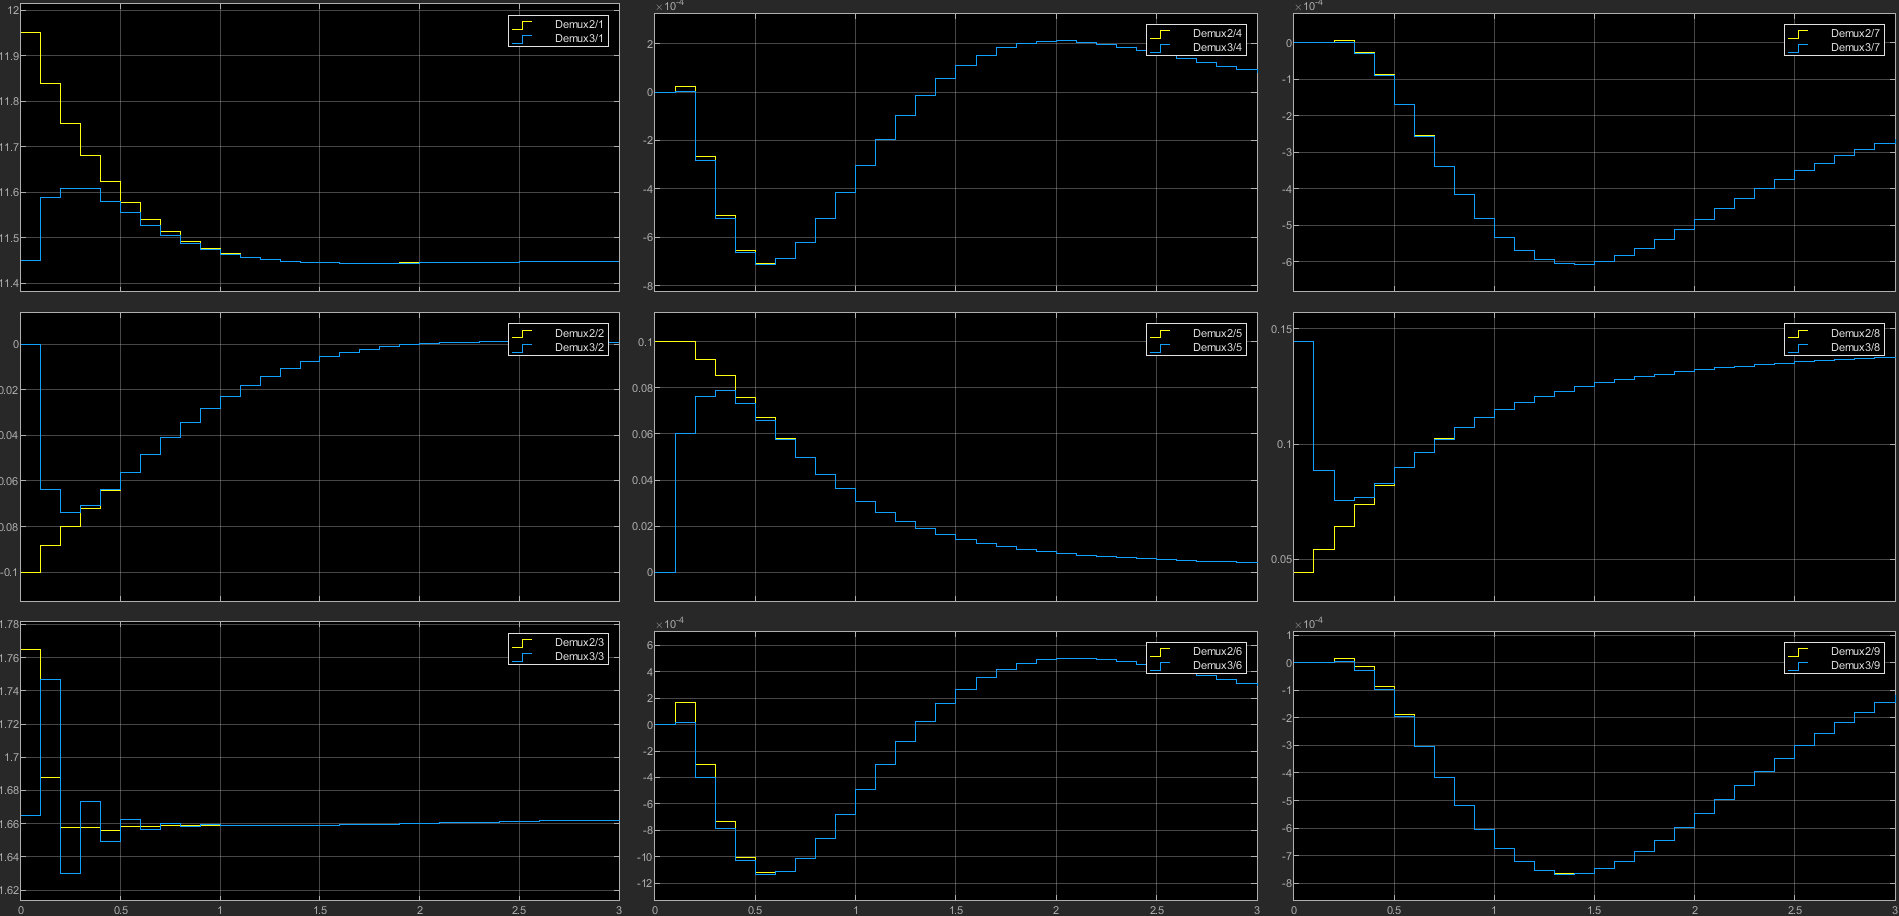
\includegraphics[width=75mm,height=50mm]{SIMULINK2.PNG}
    \caption{Results of Lauenberg estimator with initial error}\label{fig:SIMULINK2}
\end{figure}
As we can see in {\ref{fig:SIMULINK2}} all the states and estimates converge over time even with initial error.

%%%        S  S   U       U  B B       S  S    E  E E        C     T T T T T    0       O       N        N
%%%     S         U       U  B   B    S        E           C           T        I     O   O     N  N     N
%%%        S      U       U  B B        S      E  E E    C             T        I   O       O   N    N   N
%%%           S     U   U    B   B        S    E           C           T        I     O   O     N      N N
%%%     S S           U      B B      S S      E  E  E       C         T        I       O       N        N
\subsection{Noise filtering}
Kalman filtering, also known as linear quadratic estimation (LQE) in statistics
and control theory, is an algorithm that estimates a joint probability
distribution over the variables for each time-frame using a series of
measurements observed over time, including statistical noise and other
inaccuracies, and produces estimates of unknown variables that are more
accurate than those based on a single measurement alone.
\par
Since our system will make use of sensor in order to access the available
information about our aircraft, the effect of white noise might jeopardize our
task, so in order to minimize its effect onto our control strategy we will
adapt the estimator from an extended Lauenberg estimator to a Kalman filter
with a high enough amount of trust into our linear model, that would allow us to
minimize the effect of the white noise, while still achieving a null position error over
time. First we need to add white noise to the system and the readings:
\par
\begin{align}
    X(k+1)=A_{E_d}X(k)+B_{E_d}U(K)+w(k) \\
    Y(k)=C_{E_d}X(k)+r(k)
    \label{LinearDiscreteExtendedSystemWithWhiteNoiseFormula}
\end{align}
where $w(k)$ represents the random noise at the moment k applied on the system and $r(k)$ represents the random noise on the sensors at the moment k.
We will use the same definition as in {\ref{ErrorDefinition}} for the error of the system, and the goal still remains to have no position error at steady state.
But a dynamic model of the estimator is needed:
\begin{align}
    \bar{X}(k)=X_{pred}+K_k(Y(k)-C_{E_d}x_{pred})
    \label{KalmanCorrection}
\end{align}
\par
where $X_{pred}$ represent the predicted value and $K_k$ represents the Kalman
gain matrix at point k. All the other notations keep the same meaning as
before. The main advantage of the Kalman filter is the continuous recalibration
of the filter using the prediction error. The Kalman filter replaces the static
matrix L from the Lauenberg estimator with a constantly changing $K_k$ matrix
governed by the equation:
\begin{align}
    K_k=P_{pred}{C_{E_d}}^T{(C_{E_d}P_{pred}C_{E_d}+R_k)}^{-1}
\end{align}
\par
where $R$ is a previously defined matrix that is constant throughout the whole
operation, and it represents the `thrust' we put in our linear model to predict
the behavior of the real system. This recalibration happens through the matrix
$P_k$ which is calculated by the follow equation:
\begin{align}
    P_k=(I-K_{k}C_{E_d})P_{pred}{(I-K_{k}C_{E_d})}^T+K_{k}R{K_k}^T
    \label{KalmanPRecalibration}
\end{align}
\par
The last element that needs to be discussed in the Kalman algorithm, is the
predicted value $X_{pred}$ which will be calculated at each step, and used to
recalibrate the Kalman gain matrix. Together with the predicted state there
will also be a prediction of the P matrix in $P_{pred}$:
\begin{align}
    X_{pred}=A_k\bar{X}(k-1)+B_{k}u(k-1) \\
    P_{pred}=A_{k}P_{k-1}{A_k}^T+Q_{k-1}
    \label{KalmanPrediction}
\end{align}
\par
since the Kalman filter recalibrates his Gain at each step, a big initial value
of the P matrix is given in order to start from the reading and then start
filtering out the noise.
\begin{align}
    P=10I_{12\times12} \\
    Q=I_{12\times12}   \\
    R=3I_{9\times9}
    \label{MatrixValuesOfKalman}
\end{align}
\par
Note that the size of the P and Q matrix have to match the size of the state
vector, while the size of the R matrix has to match the size of the output
vector. The values of R are greater than the values of Q in order to increase
the trust we put in our model when clearing out noise.

%%%        S  S   U       U  B B       S  S    E  E E        C     T T T T T    0       O       N        N
%%%     S         U       U  B   B    S        E           C           T        I     O   O     N  N     N
%%%        S      U       U  B B        S      E  E E    C             T        I   O       O   N    N   N
%%%           S     U   U    B   B        S    E           C           T        I     O   O     N      N N
%%%     S S           U      B B      S S      E  E  E       C         T        I       O       N        N
\subsection{Linear Gaussian controller}
\par
The linear-quadratic-Gaussian (LQG) control problem is one of the fundamental
optimum control issues in control theory. It concerns linear systems driven by
additive white Gaussian noise. The objective is to identify an output feedback
rule that minimizes the expected value of a quadratic cost criteria. The
starting state is likewise regarded as a Gaussian random vector, and Gaussian
noise is meant to distort output measurements.
\par
This makes the LQG controller one of the best among the larger class of
nonlinear controllers. That is given by the fact that applying a nonlinear
control method won't make the anticipated value of the cost functional grow
into account. This variation of the separation principle is a special case of
the separation principle of stochastic control, which states that even when the
process and output noise sources are potentially non-Gaussian, the optimal
control separates into an optimal state estimator (which may no longer be a
Kalman filter) and a LQR regulator as long as the system dynamics are linear.
\par
Under these assumptions, an optimum control strategy may be created inside the
class of linear control rules using the completion-of-squares argument. The
linear-quadratic regulator (LQR) and linear-quadratic estimator (LQE) of the
Kalman filter are combined to create the unique control rule known as the LQG
controller (LQR). The state estimator and state feedback can be constructed
independently, according to the separation idea. LQG control is a
straightforward linear dynamic feedback control rule that can be computed and
applied to both linear time-invariant and linear time-varying systems. The LQG
controller is a dynamic system like the system it regulates. Both systems have
the same state dimension.
\par
Since a reliable optimal estimator has been developed we can now proceed to the
next step, namely the construction of a controller. A linear quadratic controller
is a full-state feedback controller designed with the purpose of minimize a quadratic cost function.
\par
This function is known as the quadratic cost function:
\begin{align}
    J=x^T_{(t_1)}F_{(t_1)}x_{(t_1)}+\int_{t_0}^{t_1} {(x^{T}Q_{x}+u^{T}R_{u}+2x^{T}N_{u})} \,dx
\end{align}
\par
Where $x$ is the state vector of the system, $u$ is the input vector of the system,
$F$ is the variable that will be used to minimize the cost, which in different
notations is $K$, and $R$ and $Q$ are, just like in the Kalman filter, cost matrices.
\par
\begin{figure}
    \centering
    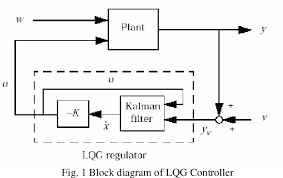
\includegraphics[width=70mm,height=50mm]{GAUSS.png}
    \caption[]{Block diagram of a Gaussian control strategy}\label{Gauss}
\end{figure}
\par
A big disclaimer of this approach is the fact that this control method
has been developed based on linear-time invariant system, and will require a level of linearization before it can be implemented onto highly non-linear systems. That is why this controller will be developed around the desired point of operation.
%%%        S  S   E  E E           C     T T T T T      0      O
%%%     S          E              C              T      I    O   O
%%%        S       E  E E    C                 T        I   O     O
%%%           S    E               C             T      I    O   O
%%%     S S       E  E  E            C        T         I      O  

\section{Course correcting}
The linear quadratic controller will ensure the stability of the system in an inner loop, even in the presence of disturbances, but it will not be able to set a course for the aircraft. In order to do that there are two options:
\par
\begin{enumerate}
    \item Adding a linear matrix, usually noted with N in the literature, that will
          linearly bind our $3\times1$ reference vector to our $5\times1$ input vector.
    \item Using a decoupled approach on the stabilized system and adding 2 independent
          controllers with proportional and integrating effects to ensure no steady-state
          error.
\end{enumerate}
\par
The latter has been chosen for this study, in order to take complete advantage of the horizontal and vertical decoupling. A feedback-based control loop known as a
proportional-integral-derivative controller (PID controller, also known as a
three-term controller), is frequently used in industrial control systems and
other applications that call for continuously modulated control. An error value
$e(t)$ is calculated by a PID controller as the difference between a desired set
point (SP) and a measured process variable (PV) on a continuous basis. A
correction is then made using terms that are proportional, integral, and
derivative (denoted P, I, and D, respectively) in nature.
\par
In reality, PID automatically corrects a control function with an accurate and
responsive adjustment. A car's cruise control, for instance, would slow down if
constant engine power was used when climbing a slope. By progressively
increasing the engine's power output, the PID algorithm in the controller
brings the recorded speed back to the desired speed with the least amount of
delay and overshoot.
\par
Since we will do this on the stabilized system, that uses a discrete time
estimator, discrete time transfer functions will be needed to define the PID controllers. We can check the
validity of this approach by looking into the stability of the transfer
function, which should reflect the stability of the linearly controlled system.
\par
First in order to define the transfer functions we can start from our state
space representation of the extended model with the linear quadratic
controller. Thus:
\begin{align}
    \dot{X(t)}=AX(t)+BU(t) \\
    Y(t)=CX(t)+DU(t)
\end{align}
\par
Applying the Laplace transformation to the linear system yields:
\begin{align}
    s{X(s)}=AX(s)+BU(s) \\
    Y(s)=CX(s)+DU(s)
\end{align}
In order to obtain the transfer function, a linear relation between $Y(s)$ and $U(s)$ needs to be defined.
\begin{align}
    sX(s)-AX(s)=BU(s) \\
    (sI-A)X(s)=BU(s)  \\
    X(s)={(sI-A)}^{-1}BU(s)
\end{align}
\par
Replacing the new form of $X$ in the output equation would yield a direct
relationship between the input and output of the system. Thus:
\begin{align}
    Y(s)=C{(sI-A)}^{-1}BU(s)+DU(s) \\
    Y(s)=(C{(sI-A)}^{-1}B+D)U(s)   \\
    H(s)=\frac{Y(s)}{U(s)}={C(sI-A)}^{-1}B+D
    \label{StateSpaceToTransferFunction}
\end{align}
\par
Since we are interested only in the position of the aircraft, and we have the
Global Positioning System available to give us the current position, we can
assume the only output of the system will be the position. Thus, The $C$ matrix
will be a $3\times12$ matrix. By using the {\ref{StateSpaceToTransferFunction}}
formula we can define the transfer function matrix $H(s)$ which is a 3-by-5
matrix containing the transfer function between the output i and the input j in
the element $H_{(i,j)}(s)$. The standard form of our transfer function will be:
\begin{align}
    H(s)=\begin{bmatrix}
             H_{1,1}(s) & H_{1,2}(s) & H_{1,3}(s) & H_{1,4}(s) & H_{1,5}(s) \\
             H_{1,1}(s) & H_{2,2}(s) & H_{2,3}(s) & H_{2,4}(s) & H_{2,5}(s) \\
             H_{1,1}(s) & H_{3,2}(s) & H_{3,3}(s) & H_{3,4}(s) & H_{3,5}(s)
         \end{bmatrix}
\end{align}
Now in order to calculate the relative gain array(RGA), the steady state gain matrix has to be calculated.
For that we only need to evaluate our system transfer function at steady state (s=0).
Since our estimator and actuators are discrete we will first use the Euler discretization technique to rewrite our transfer function matrix in the discrete time space, and evaluate it at (z=1).
So first our system will become:
\begin{align}
    H(z)=\begin{bmatrix}
             H_{1,1}(z) & H_{1,2}(z) & H_{1,3}(z) & H_{1,4}(z) & H_{1,5}(z) \\
             H_{1,1}(z) & H_{2,2}(z) & H_{2,3}(z) & H_{2,4}(z) & H_{2,5}(z) \\
             H_{1,1}(z) & H_{3,2}(z) & H_{3,3}(z) & H_{3,4}(z) & H_{3,5}(z)
         \end{bmatrix}
    \label{DiscretTimeTransferFunction}
\end{align}
By evaluating the {\ref{DiscretTimeTransferFunction}} at the point z=1 we will gain the relative gain matrix (RGA) as:
\begin{align}
    RGA=\begin{bmatrix}
            0.8245  & 0.1508 & -0.0007 & 0.0343 & -0.0089 \\
            -0.0004 & 0.0005 & 0.5646  & 0.2083 & 0.2269  \\
            0.0124  & 0.8370 & 0.0227  & 0.1101 & 0.0178
        \end{bmatrix}
\end{align}
The relative gain matrix is a matrix of influence of the inputs to the outputs.
In order to be able to safely decouple our system we are looking for the dominant members on each row.
Because the terms $(1,1)$,$(2,3)$ and $(3,2)$ are the dominant members on they're respective row, and since they are at least 5 times bigger than their counterparts, we can safely make the assumption that our system can be decoupled:
\begin{align}
    H(z)=\begin{bmatrix}
             H_{1,1}(z) & 0          & 0          & 0 & 0 \\
             0          & 0          & H_{2,3}(z) & 0 & 0 \\
             0          & H_{3,2}(z) & 0          & 0 & 0
         \end{bmatrix}
    \label{DecoupledDiscretTimeTransferFunction}
\end{align}
Which also respects the intuitive answer that the forward velocity of the aircraft is directly controller by the thrust input, the lateral velocity of the aircraft is mainly influenced by the rudder and that the vertical velocity of the aircraft is mainly controller by the elevator.
Since our aircraft is always expected to move forward we can even ignore the first row of our matrix and only develop 2 controllers for our lateral and vertical movements.

%%%        S  S    E  E E        C     T T T T T    0       O       N        N
%%%     S          E           C           T        I     O   O     N  N     N
%%%        S       E  E E    C             T        I   O       O   N    N   N
%%%           S    E           C           T        I     O   O     N      N N
%%%     S S        E  E  E       C         T        I       O       N        N
\section{Conclusion}
After decoupling our system we can finally apply our complete control a
structure on top of the non-linear model in Simulink to see the results. After
making the connections from our control structure to our model we can simulate
our system. It will be simulated on a longer time-frame with multiple
disturbances all in the form of step inputs, sprinkled along the way.
\par
\begin{figure} [h]
    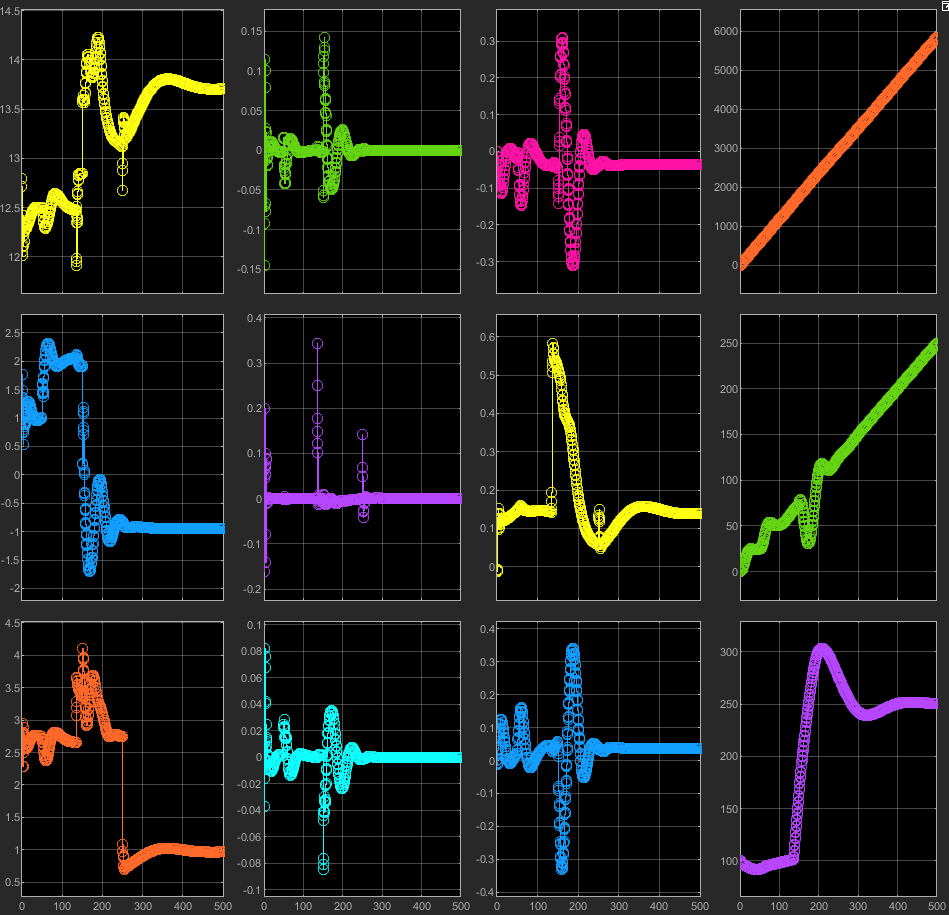
\includegraphics[width=75mm,height=50mm]{StatesSimulation.PNG}
    \caption[]{System states on simulation}\label{fig:SIMULINK6}
\end{figure}
In the figure {\ref{fig:SIMULINK6}} all the states of the system as defined in previous sections except for the wind vector.
\begin{figure} [h]
    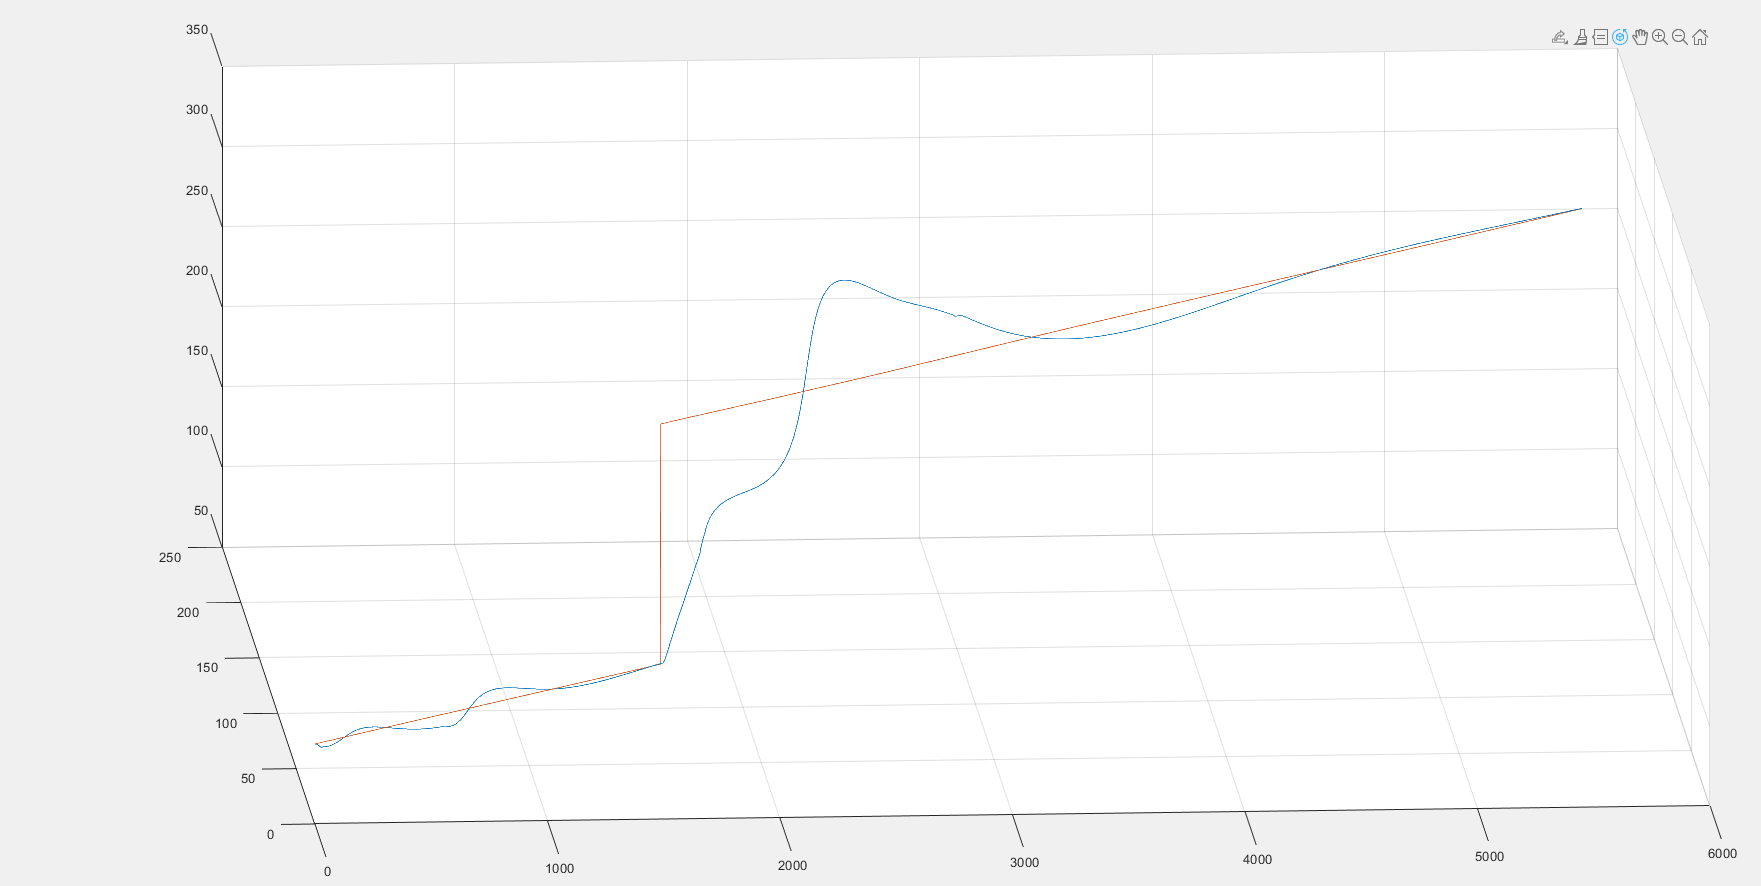
\includegraphics[width=75mm,height=50mm]{PathFollowing.PNG}
    \caption[]{Cruise flight mission simulation in 3 dimensional space}\label{fig:SIMULINK8}
\end{figure}
In the figure {\ref{fig:SIMULINK8}} the reference trajectory is displayed in a 3 dimensional space together with the real trajectory followed by the aircraft.
Both examples follow a trajectory mainly emphasizing lateral and vertical movement relative to the starting orientation.
This has been chosen because of the limitations of our implementation.

%%%        S  S   U       U  B B       S  S    E  E E        C     T T T T T    0       O       N        N
%%%     S         U       U  B   B    S        E           C           T        I     O   O     N  N     N
%%%        S      U       U  B B        S      E  E E    C             T        I   O       O   N    N   N
%%%           S     U   U    B   B        S    E           C           T        I     O   O     N      N N
%%%     S S           U      B B      S S      E  E  E       C         T        I       O       N        N
\subsection*{Achievements}
In this paper the groundwork for the development of an aircraft controller has
been developed using an optimal control approach and two proportional
integrating controllers. This approach has been developed with the scope of a
small-scale aircraft with limited computational resources which is expected to
have an automated guidance system onboard. It takes into account the size
limitations and proposes an efficient algorithm sufficient for basic cruise
control.

%%%        S  S   U       U  B B       S  S    E  E E        C     T T T T T    0       O       N        N
%%%     S         U       U  B   B    S        E           C           T        I     O   O     N  N     N
%%%        S      U       U  B B        S      E  E E    C             T        I   O       O   N    N   N
%%%           S     U   U    B   B        S    E           C           T        I     O   O     N      N N
%%%     S S           U      B B      S S      E  E  E       C         T        I       O       N        N
\subsection*{Further development}
In the future this approach could be extended to allow for fully autonomous
aircraft with the ability to perform complex areal maneuvers and be able to
land and take off safely. For this the before mentioned gain-scheduled
architecture could be used, together with a performant mission planner and more
efficient sensors for better data acquisition.
\begin{thebibliography}{20}
    \bibitem{state_estimation}
    \newblock{Thijs Devos, Matteo Kirchner, Jan Croes, Wim Desmet and Frank Naets}
    \newblock{Sensor Selection and State Estimation for Unobservable and Non-Linear System Models}
    \bibitem{Field_Path_Following_for_Miniature_Air_vehicles}
    Derek R. Nelson, BlakeBarber, Timothy W. McLain,
    \newblock{Randal W. Beard}
    \newblock{Vector Field Path Following for Miniature Air vehicles}
    \bibitem{Nonlinear_and_Adaptive_Control_Design}
    \newblock{M. Krstic, I. Kanellakopoulosand }
    \newblock{P. V. Kokotovic,}
    \newblock{\emph{Nonlinear and Adaptive Control Design}, John Wiley and Sons}
    \newblock{NewYork,1995.}
    \bibitem{Dynamics_of_Atmospheric_Flight}
    Bernard Etkin, Dynamics of Atmospheric Flight,1972.

    \bibitem{Aircraft_Control_and_Simulation}
    Brian L.
    Stevens and Frank L.
    Lewis, \emph{Aircraft Control and Simulation},2003.
    \bibitem{Equations_of_Motion}
    John W.
    Lincoln, Structures Division, Directorate of Flight Systems Engineering, \emph{Aircraft landing dynamic analysis} AD-A240 123
    \bibitem{Karman}
    de Karman, Theodore; Leslie Howarth (1938).
    \emph{On the Statistical Theory of Isotropic Turbulence}
    \bibitem{Gust}
    Diedrich, Franklin W.; Joseph A.
    Drischler (1957).
    \emph{Effect of Span wise Variations in Gust Intensity on the Lift Due to Atmospheric Turbulence}: NACA TN 3920.
    \bibitem{Wind_Sheer}
    Adrian F.
    Tuck \emph{Turbulence: Vertical Shear of the Horizontal Wind, Jet Streams, Symmetry Breaking, Scale Invariance and Gibbs Free Energy}
    \bibitem{Wind_speed}
    Michael Borsche, Andrea K.
    Kaiser-Weiss, and Frank Kaspar, \emph{Wind speed variability between 10 and 116 m height from the regional reanalysis COSMO-REA6 compared to wind mast measurements over Northern Germany and the Netherlands}
    \bibitem{51}
    J. Abzugand E. E. Larrabee, \emph{Airplane Stability and Control: A History of the Technologies that Made Aviation Possible}, Cambridge University Press,2002.
    \bibitem{Wind_profiles}
    Pryian Mendis, Tuan Duc Ngo, N.
    Haritos and Bijan Samali, \emph{Wind loading on tall buildings}, Electronic Journal of Structural Engineering · January 2007
    \bibitem{UTC}
    \newblock{Cornel-Alexandru Brezoescu}
    \newblock{\emph{Small lightweight aircraft navigation in the presence of wind}}
    \newblock{Université de Technologie de Compiègne}
    \newblock{2013. English.}
    NNT:2013 COMP 2105
    \bibitem[]{Gain_Scheduled}
    \newblock{Johannes Stephan and Walter Fichter }
    \newblock{Gain-Scheduled Multivariable Flight Control under Uncertain Trim Conditions}
    \newblock{Institute of Flight Mechanics and Control, University of Stuttgart, Germany}
    \bibitem{lessons}
    \newblock{Tor Erik Evjemo and S.}
    O. Johnsen
    \newblock{SINTEF, Trondheim, Norway.}
    E-mail: Torerik.evjemo@sintef.no
    \newblock{Lessons Learned from Increased Automation in Aviation: The Paradox Related to the High Degree of Safety and Implications for Future Research}
\end{thebibliography}
\end{document}